\section{Identifying privacy-related vulnerabilities in CWE and CVE} \label{sec:identifying-privacy-vul}

Common Weakness Enumeration (CWE) and Common Vulnerabilities and Exposures (CVE) are two well-known systems for publicly known weaknesses and vulnerabilities in software and hardware. % A vulnerability is defined as ``a weakness in an information system, system security procedures, internal controls, or implementation that could be exploited or triggered by a threat source'' \cite{Guitierrez2013}.
The CWE system identifies common categories of flaws, bugs and other errors found in software and hardware implementation, code, design or architecture that could be vulnerable to attacks \cite{CWE}. The CWE system has three views: i) by research concepts, ii) by software development and iii) by hardware design. Our study focuses on the research concepts and software development views as they are related to software applications. A CWE record consists of a description, relationships to other CWE records, demonstrative examples, mitigations and other relevant attributes. The interested parties can use this information to identify a weakness in their software systems and applications. For example, CWE-359\footnote{https://cwe.mitre.org/data/definitions/359.html} describes a weakness that exposes private personal information to an unauthorised actor (see Figure \ref{fig:cwe-359}). It also provides demonstrative examples, one of which is a code fragment that exposes a user's location. %, and specifies the potential mitigations such as identifying and consulting with all relevant privacy regulations regarding the processing of users' location.

\begin{figure}[ht]
	\centering
	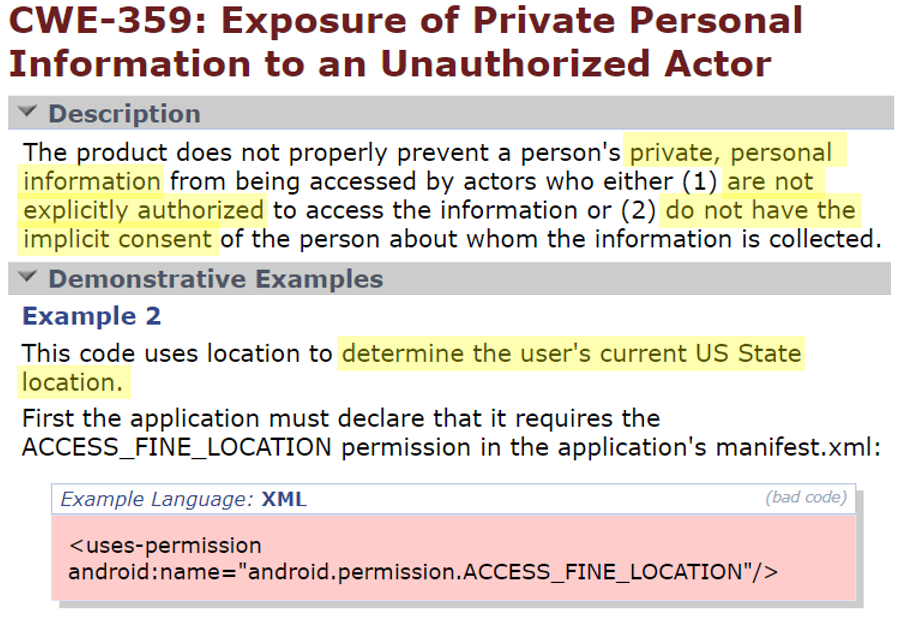
\includegraphics[width=1.0\linewidth]{figures/cwe-359.png}
	\caption{A screenshot highlights privacy-related information in CWE-359.}
	\label{fig:cwe-359}
\end{figure}

CVE is a catalogue of cybersecurity vulnerabilities that may exist in software products, applications and open libraries (e.g. Skype, Mozilla Firefox and Android). These vulnerabilities are reported by organisations that have partnered with the CVE program. Each CVE record describes the details of a vulnerability and specifies affected version of a software, thus it is more specific comparing to CWE records. For example, CVE-2000-1243\footnote{https://cve.mitre.org/cgi-bin/cvename.cgi?name=CVE-2000-1243} refers to a privacy leak in version 3.04 of Dansie Shopping Cart which sensitive information such as user credentials were sent to an e-mail address controlled by the product developers.

In the absence of a system which specifically records common privacy vulnerabilities, software engineers and other interested parties often rely on the CWE and CVE systems for privacy weaknesses and vulnerabilities (like the one in Figure \ref{fig:cwe-359}). However, both CWE and CVE target at cybersecurity, and although security and privacy are often discussed together, they are not the same. Security vulnerabilities are often exploited by unauthorised access to perform malicious actions in software applications. By contrast, privacy vulnerabilities may lead to violations of the individual rights to their personally identifiable information in terms of how those personal data are collected, used, protected, transferred, altered, disclosed and destroyed. Hence, we have explored to what extent privacy concerns are covered in the CWE and CVE systems, and whether privacy receives adequate attention which it deserves.

\subsection{Approach}

The privacy vulnerability identification process (see Figure \ref{fig:privacy-vul-identification}) consists of the following steps: (i) obtaining the CWE and CVE lists, (ii) determining a list of keywords and performing a keyword search, (iii) identifying privacy-related criteria and annotating the CWE and CVE records, and (iv) performing privacy vulnerability analysis.

\begin{figure}[ht]
	\centering
	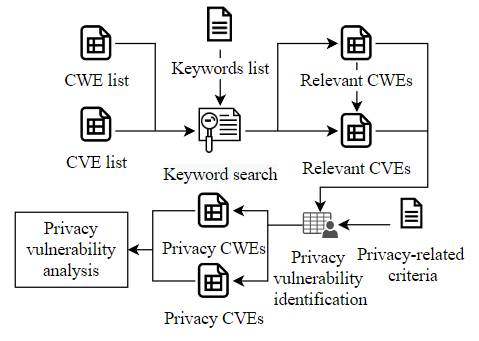
\includegraphics[width=.9\linewidth]{figures/privacy-vulnerability-identification.png}
	\caption{Privacy vulnerabilities identification process.}
	\label{fig:privacy-vul-identification}
\end{figure}

To identify the privacy vulnerability in CWE and CVE lists, we first downloaded the whole CWE records in the research concepts and software development views\footnote{The CWE data is available at https://cwe.mitre.org/data/downloads.html} and CVE records\footnote{The CVE data is available at https://cve.mitre.org/data/downloads/index.html} from their websites. We examined all the attributes of 922 weaknesses in both research concepts and software development views in the CWE to date. The CVE list contains 156,537 records to date, all of which were examined in our study. We examined all of the following attributes in each CVE record: name (i.e. CVE-ID), status, description, references, phases, votes and comments.

After obtaining both lists, we then performed keyword searches to filter out the CWE and CVE records that do not have privacy-related keywords. We used a search function in Microsoft Excel to examine the keywords in those records. A set of keywords consists of 37 words categorised into 4 groups as follows:

\begin{itemize}[leftmargin=*]
    \item Group 1: general terms that relate to weaknesses and vulnerabilities in privacy. The terms include privacy, violation, leak and leakage (4 keywords). The term \emph{privacy} generally appears in the CWE and CVE that reported privacy weaknesses and vulnerabilities. On top of that, we also include the terms \emph{violation, leak and leakage} as they are alternatively used to express concerns in the context of privacy (see CWE-359\footnote{https://cwe.mitre.org/data/definitions/359.html} for more details).

    \item Group 2: terms used to refer to personal data or personally identifiable data. They could be sometimes used interchangeably across regulations, standards and industry sources. The keywords in this group include personal information, personal data, sensitive information, sensitive data, private information, private personal information, personally identifiable information, PII, protected health information, PHI, health information and health data (12 keywords). %These terms are used in regulations (e.g. GDPR and HIPAA), standards (e.g. ISO/IEC 29100) and industry sources (e.g. Norton, CWE and CVE).

    \item Group 3: terms that relate to relevant privacy and data protection regulations/standards/frameworks. In this group, we select a set of specific well-known and widely-adopted data protection regulations and privacy frameworks mentioned in the CWE records, which includes General Data Protection Regulation, GDPR, California Consumer Privacy Act, CCPA, Health Insurance Portability and Accountability Act, HIPAA, Gramm-Leach Bliley Act, GLBA, Safe Harbor Privacy Framework, ISO/IEC 29100 (10 keywords). In addition, we also include the general terms to ensure that we cover unseen regulations and frameworks which are regulation, data protection, privacy act, privacy framework and privacy standard (5 keywords).

    \item Group 4: terms that are frequently seen in the privacy policies and literature when discussing personal data protection and user privacy. These include right(s), consent, opt in/opt-in, opt out/opt-out, preference and breach (6 keywords).
\end{itemize}

%\begin{table}
\caption{Individual rights on privacy}
\label{tab:rights}
\begin{tabular}{p{3.75cm} p{3.75cm}}
	\toprule
	Rights &
	Relevant data protection regulations/privacy acts \\ \midrule
	Right to be informed &
	GDPR, CCPA, HIPAA, GLBA, APA \\
	Right of access &
	GDPR, HIPAA, USPA, APA \\
	Right to rectification &
	GDPR, HIPAA, USPA, APA \\
	Right to erasure &
	GDPR, CCPA \\
	Right to restrict of processing &
	GDPR, HIPAA \\
	Right to data portability &
	GDPR \\
	Right to object &
	GDPR, APA \\
	Right in relation to automated decision making and profiling &
	GDPR \\
	Right to opt-out of sale &
	CCPA \\
	Right to non-discrimination &
	CCPA \\
	Right to request confidential communications &
	HIPAA \\
	Right to be protected against unwarranted invasion &
	GDPR, USPA \\
	Right to make a complaint &
	GDPR, APA \\
	Right to opt-out of sharing &
	GLBA \\
	Right to not identifying yourself &
	APA \\ \bottomrule
\end{tabular} 
\footnotesize \flushleft{\textit{GDPR: European General Data Protection Regulations, CCPA: California Consumer Privacy Act, HIPAA: Health Insurance Portability and Accountability Act, USPA, U.S. Privacy Act, GLBA: Gramm-Leach Bliley Act and APA: Australian Privacy Act.}}
\end{table}

\begin{comment}
\begin{table*}[ht]
\caption{Individual rights on privacy}
\label{tab:rights}
\begin{tabular}{p{4cm} p{10cm} p{3cm}}
\toprule
Rights &
  Description &
  Relevant data protection regulations/privacy acts \\ \midrule
Right to be informed &
  Individuals must be informed about the collection, use and processing of their personal data. For example, the software applications must inform the purposes of personal data collection and processing. In case the personal data is processed by other parties, the individuals must be informed to whom their personal data is disclosed/transferred. &
  GDPR, CCPA, HIPAA, GLBA, APA \\
Right of access &
  Individuals must be able to request to access and receive a copy of their personal data. &
  GDPR, HIPAA, USPA, APA \\
Right to rectification &
  Individuals must be able to request to correct, complete and/or make changes to their personal data. &
  GDPR, HIPAA, USPA, APA \\
Right to erasure &
  Individuals must be able to request to erase their personal data. &
  GDPR, CCPA \\
Right to restrict of processing &
  Individuals must be able to request to restrict of personal data processing. &
  GDPR, HIPAA \\
Right to data portability &
  Individuals must be able to request obtain, reuse, move, copy or transfer their personal data across different services for their own purposes. &
  GDPR \\
Right to object &
  Individuals must be able to object to the processing of their personal data in certain circumstances (e.g. direct marketing). &
  GDPR, APA \\
Rights in relation to automated decision making and profiling &
  Organisations must obtain consent from individuals when the software may process their personal data based on automated decision making and profiling. &
  GDPR \\
Right to opt-out of sale &
  Individuals must be able to request to opt-out if their personal data is sold by organisations. &
  CCPA \\
Right to non-discrimination &
  Individuals, who exercise their individual rights with respect to particular regulations, must be provided with the same quality and price of goods and services by businesses. &
  CCPA \\
Right to request confidential communications &
  Individuals must be able to request to change means or location for receiving communication of health information. &
  HIPAA \\
Right to be protected against unwarranted invasion &
  Personal data must be protected from invasion resulting from the collection, use, disclosure, maintenance and other processing. &
  GDPR, USPA \\
Right to make a complaint &
  Individuals must be able to lodge a complaint to relevant organisations or supervisory authority if their personal data is mishandled. &
  GDPR, APA \\
Right to opt-out of sharing &
  Individuals must be able to opt-out from sharing their personal data. &
  GLBA \\
Right to not identifying yourself &
  Individuals must have an option not identifying themselves in certain circumstances (e.g. using pseudonym). &
  APA \\ \bottomrule
\end{tabular}
\vspace{0.5mm}
\\
\footnotesize \flushleft{\textit{GDPR: European General Data Protection Regulations, CCPA: California Consumer Privacy Act, HIPAA: Health Insurance Portability and Accountability Act, USPA, U.S. Privacy Act, GLBA: Gramm-Leach Bliley Act and APA: Australian Privacy Act.}}
\end{table*} 
\end{comment}

We acquired 185 CWE and 1,088 CVE records that contain at least one of the specified keywords. Next, we manually examined each of those records to identify privacy vulnerabilities. A vulnerability is considered as privacy-related if it satisfies one of the following criteria:

\begin{enumerate}[leftmargin=*]
	\item A weakness or vulnerability involves with any processing of personal data (e.g. collection, use, storage, transfer, alteration, erasure and disclosure). %As personal data can be used on its own or in conjunction with other information to identify or trace an individual (e.g. name, identification number, social security number, user credentials, health records, email addresses), the processing of personal data may affect information and user privacy \cite{Scholz2015, ISO/IEC2011, DataPrivacyManager2021}.

    \item A weakness or vulnerability which may lead to the violations of the individual rights. To extract the individual rights, we first selected a range of well-established data protection and privacy regulations in different domains such as governments, businesses, healthcare and finance (i.e. EU GDPR, CCPA, HIPAA, GLBA, USPA, APA). These regulations have been widely enacted in country- and regional-level, hence they are well respected by organisations worldwide. In each regulation, we went through each article to look for the individual rights of data subjects/patients/consumers. Once we found the individual right, we added it into our list\footnote{See the file named \emph{``14-rights''} in the data folder in the replication package for the complete list of individual rights and their relevant data protection regulations/privacy acts.}.

\end{enumerate}

We went through the shortlisted 185 CWE and 1,088 CVE records to determine the vulnerabilities that meet the above criteria. In addition, we have found that the National Vulnerability Database (NVD) had done some mapping between CVEs and CWEs. Hence, once we have identified privacy-related CVEs, we used this mapping and applied the above criteria to identify additional privacy-related CWE records.

%We also note that the CWE weaknesses are organised hierarchically where each CWE weakness can have other CWE weaknesses as its parents or children. We investigated whether privacy properties are inherited through this structure. We discuss here CWE-200\footnote{https://cwe.mitre.org/data/definitions/200.html} as an example to demonstrate this case. CWE-200 describes a weakness that exposes sensitive information to an unauthorised actor. This weakness has one parent and eleven children. CWE-200 itself is classified as privacy-related, however its parent and seven of its children are not privacy-related. Similarly, CWE-201, one of the CWE-200 children, is privacy-related, but its child CWE-598 is not privacy-related. We also further explored the rest of CWE-200 children, and found that privacy properties are not inherited through the hierarchical structure. Thus, we did not take a hierarchical structure into account when examining whether a weakness is privacy-related.

\subsection{Results}

We identified 41 and 157 privacy vulnerabilities in the CWE and CVE records respectively. The first 28 privacy-related CWE records were found after the keyword search and manual examination steps. The additional 13 privacy-related CWE records were later added after being identified by the privacy-related CVE records. They cover a wide range of privacy concerns in software applications such as missing personal data protection, improper access control, insufficient credentials protection and personal data exposures. These weaknesses and vulnerabilities are not only related to security, but also affect privacy of individuals.

% unintentional errors made by software developers and personal data attacks from external attackers. These weaknesses and vulnerabilities are not only related to security, but also affect privacy of individuals. %Thus, privacy should gain more attention in this CWE and CVE systems as software developers refer to both systems when developing software systems.

We discuss here a few examples of CWE and CVE records that were classified as privacy vulnerabilities or weaknesses and refer the reader to \cite{rep-pkg-privul} for a full list of them. CWE-359\footnote{https://cwe.mitre.org/data/definitions/359.html} refers to the exposure of private personal information to an unauthorised actor. Private personal information here includes social security numbers, geographical location, financial data and health records. In addition, this CWE also mentions relevant data protection regulations and privacy acts such as GDPR and CCPA.

Another example is CVE-2020-13702\footnote{https://cve.mitre.org/cgi-bin/cvename.cgi?name=CVE-2020-13702} which refers to the rolling proximity identifier used in the Apple/Google exposure notification API beta through 2020-05-29. This vulnerability enables attackers to evade Bluetooth Smart Privacy due to a secondary temporary UID through tracking individual device movement using a Bluetooth LE discovery mechanism. This is a privacy vulnerability since it concerns user's location and relates to the processing of user's location. There are many cases where the reported vulnerabilities are \emph{not} specifically privacy-related. For example, CWE-78\footnote{https://cwe.mitre.org/data/definitions/78.html} enables the attacker to execute arbitrary commands on the operating systems, leading to unauthorised access to operating systems. However, this is not specifically a privacy vulnerability since it does not involve personal data, personal data processing or individual rights. 

%CVE-2021-21301\footnote{https://cve.mitre.org/cgi-bin/cvename.cgi?name=CVE-2021-21301} describes a vulnerability in Wire for iOS (iPhone and iPad) before version 3.75. The application enables camera for video capturing, although the users have disabled this service. This vulnerability seriously violates user privacy as the users are not aware of their camera being enabled, and the camera may capture and expose the users and their environment.

%CVE-2019-16522\footnote{https://cve.mitre.org/cgi-bin/cvename.cgi?name=CVE-2019-16522} refers to the cross-site scripting (XSS) attacks occurred in WordPress. The eu-cookie-law plugin through 3.0.6 for WordPress is vulnerable to cross-site scripting (XSS) attacks. This vulnerability affects the cookie consent message which leads to the unclear information provided to the users, including details regarding personal data processing. CVE-2011-1717\footnote{https://cve.mitre.org/cgi-bin/cvename.cgi?name=CVE-2011-1717} describes a vulnerability occurred in Skype for Android. The application stores sensitive user data without encryption in the sqlite3 databases (e.g. user IDs, phone number and date of birth). This CVE concerns the user data that can be used to identify an individual such as phone number and date of birth. It also involves with the lack of personal data protection stored in the database.

%Similarly, CVE-2021-21466\footnote{https://cve.mitre.org/cgi-bin/cvename.cgi?name=CVE-2021-21466} describes a vulnerability that allows an attacker to inject malicious code into certain versions of SAP Business Warehouse and SAP BW/4HANA. The attacker could create a malicious ABAP report which could be used to access data and disrupt the system functionalities. This vulnerability can lead to the Denial of Service. This is again a security vulnerability rather than a privacy one since it is not directly related to violations of any individual rights to their personally identifiable information.

\begin{conclusion}
	\textbf{The coverage of privacy-related vulnerabilities in both CWE and CVE records is quite limited: 4.45\% in the CWE system and 0.1\% in the CVE system.}
\end{conclusion}